\documentclass[11pt,letterpaper]{article}
\usepackage[margin=1.0in]{geometry}
\usepackage[utf8]{inputenc}
\usepackage{cite}
\usepackage{amsmath}
\usepackage{amsfonts}
\usepackage{amssymb}
\usepackage{makeidx}
\usepackage{graphicx}
\usepackage{hyperref}
\setlength\parindent{0pt}

\author{STUDENT NAME}
\title{HW6: Wien bridge derivation}

\begin{document}

\maketitle

\textbf{Introduction}

Given is the Wien bridge that is used to measure the capacitance, and series resistance of a capacitor as shown in Figure \ref{fig:HW6_WienBridge}. In addition, the frequency of the input signal can be determined. Here are the equations given that the bridge is in balance:

\begin{figure}
\centering
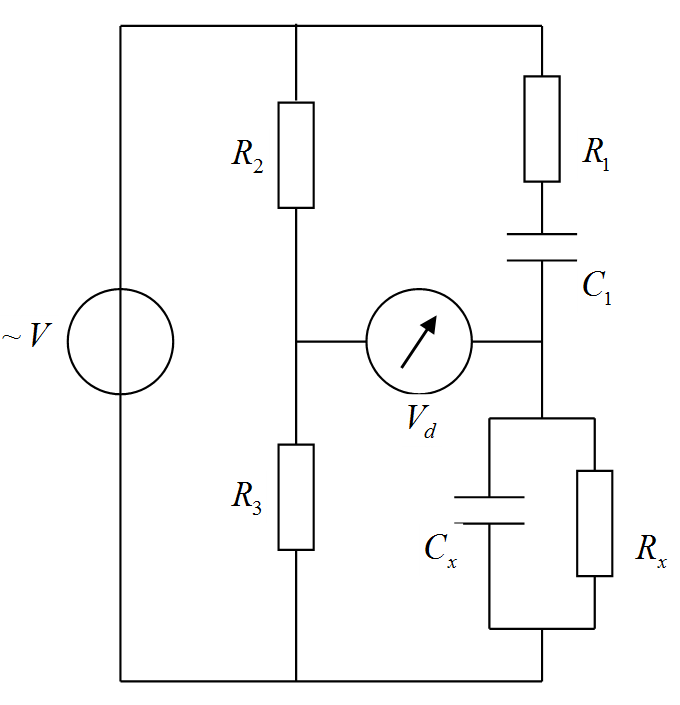
\includegraphics[width=0.7\linewidth]{HW6_WienBridge}
\caption{Wien bridge schematic.}
\label{fig:HW6_WienBridge}
\end{figure}


\begin{align}\label{HW_WienBridge1}
Z_2 &= R_2\\
Z_x &= \dfrac{R_x \dfrac{1}{j \omega C_x}}{R_x + \dfrac{1}{j \omega C_x}} = \dfrac{R_x}{1+j \omega R_x C_x}\\
Z_3 &= R_3\\
Z_1 &= R_1 + \dfrac{1}{j \omega C_1} = \dfrac{1+j \omega R_1 C_1}{j \omega C_1}\\ 
\end{align}

Here is the answer: YOUR JOB IS TO DERIVE THESE EQUATIONS BASED ON THE ONES GIVEN ABOVE.

\begin{align}\label{HW_WienBridge2}
\omega ^2 &= \dfrac{1}{R_1 C_1 R_x C_x}\\
R_x &= R_3\left( \dfrac{1 + \omega^2 R_1^2 C_1^2}{\omega^2 R_1 R_2  C_1^2} \right)\\
C_x &= \dfrac{R_2 C_1}{R_3\left( 1 + \omega^2 R_1^2 C_1^2 \right)}\\ 
\end{align}


\end{document}